% Options for packages loaded elsewhere
\PassOptionsToPackage{unicode}{hyperref}
\PassOptionsToPackage{hyphens}{url}
%
\documentclass[
]{ltjarticle}
\usepackage{lmodern}
\usepackage{amssymb,amsmath}
\usepackage{ifxetex,ifluatex}
\ifnum 0\ifxetex 1\fi\ifluatex 1\fi=0 % if pdftex
  \usepackage[T1]{fontenc}
  \usepackage[utf8]{inputenc}
  \usepackage{textcomp} % provide euro and other symbols
\else % if luatex or xetex
  \usepackage{unicode-math}
  \defaultfontfeatures{Scale=MatchLowercase}
  \defaultfontfeatures[\rmfamily]{Ligatures=TeX,Scale=1}
\fi
% Use upquote if available, for straight quotes in verbatim environments
\IfFileExists{upquote.sty}{\usepackage{upquote}}{}
\IfFileExists{microtype.sty}{% use microtype if available
  \usepackage[]{microtype}
  \UseMicrotypeSet[protrusion]{basicmath} % disable protrusion for tt fonts
}{}
\makeatletter
\@ifundefined{KOMAClassName}{% if non-KOMA class
  \IfFileExists{parskip.sty}{%
    \usepackage{parskip}
  }{% else
    \setlength{\parindent}{0pt}
    \setlength{\parskip}{6pt plus 2pt minus 1pt}}
}{% if KOMA class
  \KOMAoptions{parskip=half}}
\makeatother
\usepackage{xcolor}
\IfFileExists{xurl.sty}{\usepackage{xurl}}{} % add URL line breaks if available
\IfFileExists{bookmark.sty}{\usepackage{bookmark}}{\usepackage{hyperref}}
\hypersetup{
  pdftitle={保険市場と情報の非対称性},
  pdfauthor={アンダーランド ジェイク; 村上真緒; 鬼頭秀明},
  hidelinks,
  pdfcreator={LaTeX via pandoc}}
\urlstyle{same} % disable monospaced font for URLs
\usepackage[top=0cm, margin=3cm]{geometry}
\usepackage{graphicx,grffile}
\makeatletter
\def\maxwidth{\ifdim\Gin@nat@width>\linewidth\linewidth\else\Gin@nat@width\fi}
\def\maxheight{\ifdim\Gin@nat@height>\textheight\textheight\else\Gin@nat@height\fi}
\makeatother
% Scale images if necessary, so that they will not overflow the page
% margins by default, and it is still possible to overwrite the defaults
% using explicit options in \includegraphics[width, height, ...]{}
\setkeys{Gin}{width=\maxwidth,height=\maxheight,keepaspectratio}
% Set default figure placement to htbp
\makeatletter
\def\fps@figure{htbp}
\makeatother
\setlength{\emergencystretch}{3em} % prevent overfull lines
\providecommand{\tightlist}{%
  \setlength{\itemsep}{0pt}\setlength{\parskip}{0pt}}
\setcounter{secnumdepth}{-\maxdimen} % remove section numbering
\usepackage{amsmath}
\usepackage{color}
\usepackage{hyperref}
\usepackage{luatexja}

\title{保険市場と情報の非対称性}
\author{アンダーランド ジェイク \and 村上真緒 \and 鬼頭秀明}
\date{2022-01-17}

\begin{document}
\maketitle

近年の新型コロナウィルスの流行とその経済への打撃,地球温暖化に促された異常気象の発生は,個人の生活に潜み,努力ではどうしようもできないリスクの存在を思い知らせる.こうしたリスクを軽減する商品こそ保険である.医療保険,失業保険,災害保険の需要はこの先高まるばかりである.こうした保険は有事への富の譲渡であり,生活を送る上で大切な財であるが,保険市場に付随する問題として情報の非対称性を忘れてはいけない.以下では,保険市場に関する正誤問題を通し,保険市場に内在する情報の非対称性の問題を考える.

\begin{enumerate}
\item ある保険会社の例を考える.この保険会社は,事故の際に全額を保障する保険$A$を高い保険料$P_A$で売っている.不注意な運転をしがちな消費者は,この保険に契約している.注意深い運転をする消費者は,保険$A$の全額保障という保険内容に魅力を感じているが,保険料$P_A$が高すぎるので契約していない.これに対し,保険会社は新たな保険$B$を,安い保険料$P_B$での提供を始めた.保険$B$は事故による損害の半分までしか保障しないが,$A$より安いので,注意深い運転をする消費者はみな$B$に契約した.この状態の市場では全ての個人が保障されており,効率的である.

\item 医療保険の会社が契約時に契約者の健康状態を人間ドックを行って高い精度で把握することができれば,保険取引市場での情報の非対称性が解消され,特に政府による介入や是正措置を必要とせずに保険取引が効率的なものとなる.

\item 保険は,ある確率的な状態にのみ金銭が手に入るという点で,普通の財とは異なるといえる,また,リスク回避的な消費者にとって有事の際に受け取る保険金は平常時に収める保険料より価値が高いが,企業にとってはこの権利の便益はその期待値(保険料 - 有事の発生確率$\times$保険金)と等しくなる.

\item 保険市場における情報の非対称性による非効率性は下のFigure1のように図示できる.この市場で特徴的なのは,限界費用曲線(MC)が下向きである,つまり価格が下がるにつれて限界費用が下がるということだ.理由としては,高いリスクを有している個人ほど保険に価値を見出すので,保険が高くても買う傾向にあるからである.結果として,保険の価格が高いと高リスクの個人(保険会社にとって保障する費用が高い個人)が主に保険を購入し,保険の価格が安いと低リスクの個人(保険会社にとって保障する費用が低い個人)の購入が増えるため,限界費用曲線は図のように下向きとなる.すると,平均費用曲線(AC)が限界費用曲線より上の位置にある.企業は平均費用曲線と需要曲線(Demand)の交差までは利益を正に保つことができるが,それ以降は一個の商品の売り上げ(価格)がそれを提供する平均的な費用を下回ってしまうため企業が赤字となる.よって,保険会社は$Q_{eqm}$以下を提供する.しかし,限界費用が需要曲線を下回っている部分が存在しているのに,そこの取引が行われないため,限界費用と限界便益が一致せず市場に非効率性が生じる.

\end{enumerate}
\center{Figure1}

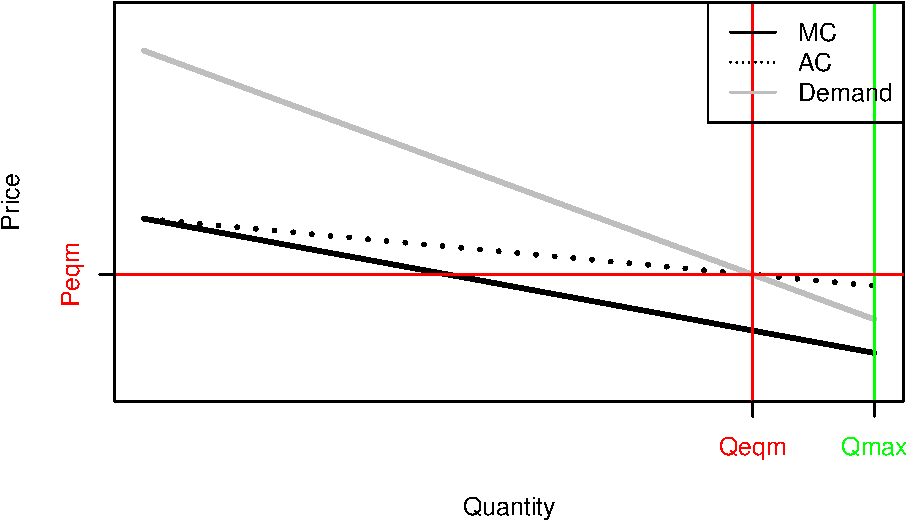
\includegraphics{group-report2_files/figure-latex/unnamed-chunk-3-1.pdf}

\newpage

\hypertarget{ux6a21ux7bc4ux89e3ux7b54}{%
\section{模範解答}\label{ux6a21ux7bc4ux89e3ux7b54}}

\begin{enumerate}

\item 誤り.この場合,注意深い消費者の第一希望は$A$であり,また保険会社は$A$は注意深い運転者にはより安い価格で$A$を提示できるのに,それをせずに注意深い運転者が妥協して$B$に契約しているため,非効率性が生じている.効率的な解決は,$A$の保険の内容をかえず,保険料だけ分別することである.実際,このような2つの保険の両立は,$A$の保険から$B$の保険への注意深いタイプの移動を招き,その結果$A$に不注意な契約者が集まり,$P_A$が上がり,また$A$から人が離れるというスパイラルが生じる可能性がある.これをデススパイラルといい,完全なる逆選択に至ると$A$の保険が提供されなくなる.

\item 誤り.たとえそうしたとしても,モラルハザードの問題が残る.保険会社は契約者の健康状態を把握するために大きなコスト(人間ドック)を割いているので,これを継続的に行うのは現実的じゃない.しかし,モラルハザードに起因する情報の非対称性を抑えるためには,瞬時に被保険者の健康状態を把握できることと,契約が継続的であることが求められるので,契約時の人間ドックのみでは非効率性は解消されない.

\item 誤り.実際には情報の非対称性が存在し,売り手と買い手が平等に有事の発生確率を把握していない.そのため,企業が確率を見誤り,実際の便益と期待値に差が生じることがある.また,財を購入する人は保険加入によって有事においても便益を得ることができるので有事を忌避する姿勢が緩くなり,有事の発生確率を上昇させることがある(モラルハザード).結果として企業は便益が常に財を販売した際の期待値と等しくなることはなく,損をすることもある.

\item 正しい.
\end{enumerate}

\end{document}
